\documentclass[a4paper,12pt,openany]{report}

\usepackage{authblk}
\usepackage{hyperref}
\usepackage{graphicx}
\usepackage[toc,page]{appendix}
\usepackage{float}               % Pour contrôler la position des figures
%French-specific commands
%--------------------------------------
\usepackage[french]{babel}
\usepackage[autolanguage]{numprint} % for the \nombre command
\usepackage{titlesec}
\hypersetup{
    colorlinks,
    citecolor=black,
    filecolor=black,
    linkcolor=black,
    urlcolor=black
}

\renewcommand{\appendixname}{Annexe} % pour le nom des chapitres individuels
\renewcommand{\appendixpagename}{Annexes} % pour le titre global de la page des annexes
\renewcommand{\appendixtocname}{Annexes} % pour le titre dans la table des matières

\titleformat{\chapter}[display]
    {\normalfont\huge\bfseries} % Style de titre
    {} % Préfixe vide
    {0pt} % Espacement entre le titre et le contenu
    {\huge} % Style du titre



\title{Rapport Projet réseaux}
\author{
    Lucas BÉRANGER \and
    Gillian LE PÉVÉDIC \and
    François BESNARD \and
    Alexandre FLOURY \and
}
\date{30/10/2024}

\begin{document}

    \maketitle  
    \newpage

    \tableofcontents
    \newpage
    \listoffigures

    \chapter{Introduction}
        \section{Présentation de l'équipe}  
            Notre équipe est composée de 4 membres, Lucas Béranger, Gillian Le Pévédic, François Besnard et Alexandre Floury..

        \section{Répartition des tâches}
            Lors de ce projet, nous nous sommes réparties les tâches de la manière suivante :
            \begin{itemize}
                \item Lucas Béranger : Configuration des services communs
                \item Gillian Le Pévédic : Configuration des VLANs sur les Switches
                \item François Besnard :  Configuration du routeur servant de Box, du Firewall et de la DMZ
                \item Alexandre Floury : Configuration du serveur DHCP
            \end{itemize}

            En résumé, voici la répartition des machines virtuelles sur les machines de TP:
            \begin{figure}
                \centering
                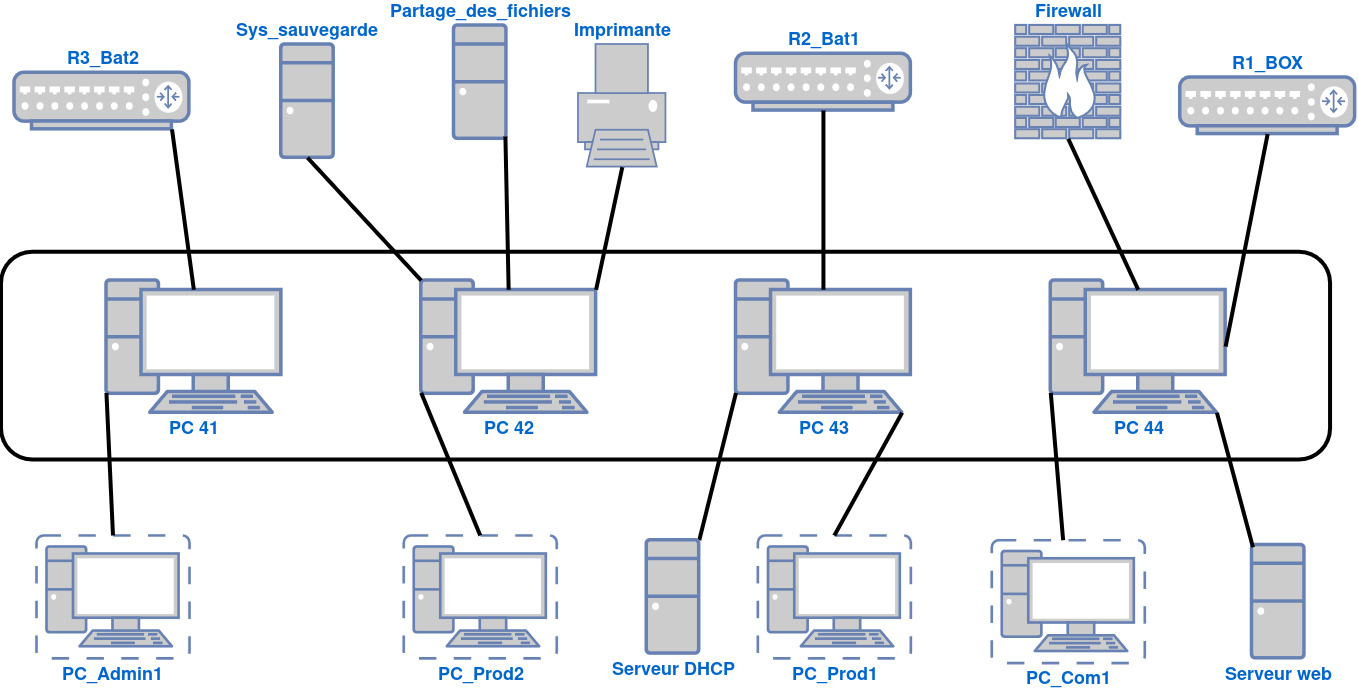
\includegraphics[width=1.2
                \textwidth]{Images/repartitions_machines.jpg}
                \caption{Répartition des machines virtuelles}
            \end{figure}

            Dans l'ordre de gauche à droite, les machines virtuelles sont respectivements celles de : Gillian, Lucas, Alexandre et François.

    \chapter{Architecture du réseau}
    \section{Le Routeur}
    Au sein du projet, le routeur qui permet de faire transiter les paquets entre les différents VLANs est une machine virtuelle sous Ubuntu. Cette machine est équipée de deux interfaces réseaux, une pour chaque bâtiment. Pour que les paquets transitent correctement entre les différents VLANs, il a ainsi fallu configurer les interfaces réseaux de la machine virtuelle pour qu'elle puisse gérer les différents VLANs.
        \subsection{Configuration}
        Pour configurer les interfaces réseaux de la machine virtuelle, il a fallu utiliser les commandes ip link. Voici un exemple de configuration pour la VM qui nous sert de routeur :
        \begin{verbatim}

    sudo ip link set enp0s9 up
    sudo ip link add link enp0s9 name enp0s9.10 type vlan id 10 
    sudo ip addr add 192,168,10,254 dev enp0s9.10 
    sudo ip link set enp0s9.10 up
        \end{verbatim}
        Il faut démarrer l'interface que l'on souhaite utiliser, puis créer une interface virtuelle pour chaque VLAN que l'on souhaite gérer. Il faut répéter cette configuration pour chaque VLAN que l'on souhaite gérer sur la machine virtuelle en veillant bien à modifier l'interface quand elle doit être modifier. 
        \subsection{Relai DHCP}
        Pour que les machines des différents VLANs puissent obtenir une adresse IP, il a fallu configurer la machine virtuelle pour qu'elle fasse office de relai DHCP. Pour cela, il a fallu installer le service isc-dhcp-relay et configurer le fichier /etc/default/isc-dhcp-relay pour qu'il pointe vers le serveur DHCP.
        \begin{verbatim}
    # What servers should the DHCP relay forward requests to?
    SERVERS="192.168.50.250"

    # On what interfaces should the DHCP relay (dhrelay) serve DHCP requests?
    INTERFACES="enp0s9.10"
        \end{verbatim}
        Le relai DHCP pointe ainsi vers le serveur DHCP qui est sur le VLAN 50 et transmettra les requêtes DHCP des différents VLANs vers le serveur DHCP.
        \section{DHCP}
            Dans les consignes, il était demandé de mettre en place un service DHCP qui permettait de fournir une adresse IP à toutes les machines du réseau. 
            
            Pour cela, le service isc-dhcp-server est déjà présent sur les distributions Ubuntu.
            \subsection{Configuration serveur}
            Pour configurer le serveur DHCP, il faut modifier le fichier /etc/dhcp/dhcpd.conf. 
            Dans ce fichier, chaque sous-réseaux/vlans doit être déclaré comme suit :
                

    \begin{verbatim}
    #Production
    subnet 192.168.10.0 netmask 255.255.255.0 {
        range 192.168.10.1 192.168.10.250;
        option routers 192.168.10.254;
        option broadcast-address 192.168.10.255;
    }
    \end{verbatim}

                
            Ici, le sous-réseau Production a une plage d'adresse allant de 192.168.10.1 jusqu'à 192.168.10.250 et une passerelle par défaut à 192.168.10.254.

            Il a été choisi de partir sur des plages d'adresses de 250 adresses pour chaque sous-réseau, ce qui fait qu'il y a un maximum de 250 machines par sous-réseau, 3 adresses sont gardées en réserve.
            Tous les sous-réseaux Commercial, Administration, Production et la DMZ sont des classes C et ont été configurés de la même manière avec leur plage d'adresses correspondant à leur vlan respectif.

            Certaines machines doivent reçevoir la même adresse IP à chaque fois qu'elles se connectent au réseau (par exemple le serveur web).
            Pour cela, il faut déclarer des machines en utilisant leur adresse MAC dans le fichier de configuration du serveur DHCP comme suit:

            \begin{verbatim}
            #Serveur Web
            host ServeurWeb {
                hardware ethernet 08:00:a0:24:21:02;
                fixed-address 192.168.100.250;
            }
            \end{verbatim}

            Avec cette partie du fichier, la machine Serveur Web reçevra toujours l'adresse IP 192.168.100.250.

            Une fois le fichier de configuration édité, il faut redémarrer le service DHCP pour que les modifications soient prises en compte:
            \begin{verbatim}
            'sudo systemctl restart isc-dhcp-server'
            \end{verbatim}
            et vérifier le status du service pour s'assurer qu'il fonctionne correctement:
            \begin{verbatim}
            'sudo systemctl status isc-dhcp-server'
            \end{verbatim}

            \subsection{Configuration DHCP client}
            Pour configurer un client et lui faire récupérer une adresse IP via le serveur DHCP, il suffit de modifier le fichier /etc/network/interfaces en ajoutant les lignes suivantes:
            \begin{verbatim}
            #Exemple avec une interface enp0s3
            auto enp0s3
            iface enp0s3 inet dhcp
            \end{verbatim}

            Si plus tard il y a besoin d'ajouter une nouvelle interface, il suffit de rajouter les lignes ci-dessus en changeant le nom de l'interface.
            Si le serveur est correctement configuré ainsi que le réseau, il reste à exécuter '\textbf{sudo dhclient}' afin de forcer le client à demander une adresse IP au serveur DHCP.
            Une fois l'exécution de la commande terminée, la commande '\textbf{ip a}' permet de vérifier que le client a bien reçu une adresse IP.

        \section{Firewall}
            \subsection{Configuration}
            Nous avons choisi de mettre en place un firewall sur notre réseau pour sécuriser les communications entre les différents VLANs. Pour cela, nous avons utilisé le service iptables présent sur les distributions Ubuntu.
            Le firewall est configuré sur la VM qui nous sert de routeur et qui permet de faire transiter les paquets entre les différents VLANs. Nous sommes partis d'une base qui refuse tout le trafic et nous avons autorisé uniquement les communications que nous souhaitions.

            \subsection{Règles}
            Pour cela nous avons mis en place un certains nombres de règles. L'un des objectifs était d'empêcher les communications entre les différents VLANs. Pour cela, nous avons mis en place les règles suivantes :
            \begin{verbatim}
iptables -A FORWARD -s 192.168.10.0/24 -d 192.168.20.0/24 -j DROP
iptables -A FORWARD -s 192.168.10.0/24 -d 192.168.60.0/24 -j DROP
iptables -A FORWARD -s 192.168.20.0/24 -d 192.168.10.0/24 -j DROP
iptables -A FORWARD -s 192.168.20.0/24 -d 192.168.60.0/24 -j DROP
iptables -A FORWARD -s 192.168.60.0/24 -d 192.168.10.0/24 -j DROP
iptables -A FORWARD -s 192.168.60.0/24 -d 192.168.20.0/24 -j DROP
            \end{verbatim}
            Nous avons également mis en place des règles pour autoriser les communications entre les différents VLANs à communiquer avec le vlan contenant tous les services communs. Tous les VLANs ont également la possibilité de communiquer avec la DMZ via des requêtes HTTP et HTTPS et sont également autorisés à communiquer avec internet via le NAT. Internet dans notre projet étant représenté par une VM a l'extérieur du réseau. 

        \section{Configuration des Switches et Réseaux VLAN}

            \subsection{VLAN (Virtual Local Area Network)}
                Les VLANs (Virtual Local Area Networks) permettent de segmenter le réseau en sous-réseaux logiques distincts au sein d'une même infrastructure physique. En assignant des ports de switch à différents VLANs, il est possible de créer des réseaux indépendants, ce qui améliore la sécurité et limite la diffusion de paquets broadcast aux appareils d'un même VLAN. Par exemple, les départements \texttt{Production}, \texttt{Commercial}, et \texttt{Administration} peuvent être assignés respectivement aux VLANs 10, 20, et 30, permettant ainsi une séparation logique de leurs flux réseau.

                La configuration de VLANs se fait en assignant une \texttt{VLAN ID} spécifique aux ports du switch souhaités. Un switch peut gérer plusieurs VLANs, chacun étant isolé des autres, sauf si une communication inter-VLAN est mise en place via un routeur ou un switch de niveau 3.

            \subsection{Trunk}
                Le mode trunk est utilisé pour permettre à plusieurs VLANs de traverser un lien unique entre deux switches. Les liens trunk encapsulent les paquets des différents VLANs avec un identifiant (généralement via l'encapsulation IEEE 802.1Q), permettant ainsi de transporter les données de plusieurs VLANs sur un même câble.

                Dans notre infrastructure, les ports configurés en mode trunk assurent la liaison entre les switches des deux bâtiments, transportant les VLANs 10, 20, 50, 60 et 100. Cette configuration permet aux différents VLANs de rester interconnectés d'un bâtiment à l'autre tout en restant isolés les uns des autres au niveau logique. 

                Pour configurer un port en mode trunk, nous utilisons la commande suivante sur un switch Cisco :

                \begin{verbatim}
interface f0/8
switchport mode trunk
switchport trunk allowed vlan 10,20,50,60,100
no shutdown
                \end{verbatim}

            \subsection{Redondance entre bâtiments}
                Afin d'assurer la continuité de service en cas de panne de lien entre les bâtiments, nous avons mis en place une redondance en utilisant des liens supplémentaires entre les switches principaux de chaque bâtiment. En cas de défaillance du lien principal, le trafic peut emprunter un lien secondaire pour maintenir la communication entre les VLANs des deux bâtiments. Cette redondance améliore la résilience de notre infrastructure et minimise les interruptions réseau en cas de défaillance matérielle ou de câble.

            \subsection{Spanning Tree Protocol (STP)}
                Le Spanning Tree Protocol (STP) est un protocole de niveau 2 conçu pour éviter les boucles de réseau dans les topologies redondantes. Lorsque plusieurs chemins sont disponibles entre les switches, STP désactive temporairement certains de ces chemins, formant un arbre sans boucle entre les switches connectés. 

                Dans notre réseau, STP détecte automatiquement les boucles potentielles entre les liens des bâtiments et désactive les chemins redondants au besoin, tout en gardant une connexion de secours disponible. Cela permet de prévenir la saturation du réseau et les tempêtes de broadcast.

                La configuration STP est souvent automatique sur les switches modernes, mais elle peut être optimisée en configurant les priorités des switches pour décider lequel sera le root bridge. Voici un exemple de commande pour configurer la priorité d'un switch :

                \begin{verbatim}
    spanning-tree vlan 10 priority 4096
                \end{verbatim}

                En abaissant la priorité d'un switch pour un VLAN donné, on peut le forcer à devenir le root bridge pour ce VLAN, ce qui optimise le chemin entre les switches.

            \subsection{Résumé}
                En résumé, l'utilisation des VLANs permet une segmentation efficace du réseau, tandis que le mode trunk facilite le transport des VLANs sur les liens entre switches. La redondance entre bâtiments améliore la résilience, et le protocole STP permet de gérer les boucles, garantissant ainsi une infrastructure réseau stable et performante.


        \section{Services Communs}
            \subsection{Système de partage de fichiers}
                Le partage de fichier permet aux utilisateurs de stocker et d'accéder à des fichiers sur un serveur centralisé. Dans notre cas pour simplifier sa mise en place, nous avons simplement installé un serveur ftp sur le serveur de production via le service vsftpd. Ce service permet de partager des fichiers entre les différents utilisateurs du réseau.
            \subsection{Système de sauvegarde}
                La sauvegarde des données est un élément essentiel de toute infrastructure informatique. En cas de panne matérielle, de corruption de données ou de sinistre, les sauvegardes permettent de restaurer les données et de minimiser les pertes. Pour notre infrastructure, nous avons pour des raison de simplicité mis en place un serveur ftp via le service vsftpd sur le serveur de production.
        \section{Serveur Web et DMZ}
            \subsection{Serveur Web}
                Le serveur web contient les pages web de l'entreprise et est accessible depuis Internet. Il permet de présenter l'entreprise, ses services et ses produits aux clients potentiels. Le serveur web est hébergé sur une machine virtuelle dans la DMZ et est accessible depuis l'extérieur via le protocole HTTP et HTTPS.
            \subsection{DMZ}
                La DMZ (Demilitarized Zone) est une zone tampon située entre le réseau interne et le réseau externe (Internet). Elle permet d'isoler les services exposés au public, tels que les serveurs web, les serveurs de messagerie ou les serveurs DNS, des réseaux internes. Sur ce réseau, la DMZ est représentée par une machine virtuelle qui héberge un serveur web accessible depuis Internet. Cette machine est connectée à un VLAN spécifique qui la sépare du reste du réseau interne et les règles de filtrage du firewall permettent de contrôler les communications entre la DMZ et les autres VLANs.
    \chapter{Conclusion}
        \section{Difficultés rencontrées}

            Lors de la mise en place de l'infrastructure, nous avons du faire face à plusieurs difficultés qui ont ralenti notre progression. Parmi les problèmes rencontrés, nous pouvons citer :

            \begin{itemize}
                \item \textbf{Préconfiguration des switchs}: Certains switchs avaient déjà une configuration préexistante. Ces configurations entravaient la mise en place de notre architecture réseau et ont nécessité une renitialisation complète des switchs.
                \item \textbf{Cables défectueux}: Certains câbles ethernet étaient défectueux, ce qui a causé des problèmes de connectivité entre les équipements. Ces câbles ont du être remplacés pour assurer une connexion stable.
                \item \textbf{Problèmes de source inconnu}: Il nous est arrivé de rencontrer des problèmes de connectivité entre les équipements sans raison apparente. En effet une machine rencontrais de problèmes lors des différents ping, la majorité des paquets étaient perdus. Après plusieurs heures de recherche, nous avons fait la conclusion qu'il s'agissait d'un problème matérielle.
                \item \textbf{Problèmes de configuration}: Initialement, la configuration des vlan sur la VM qui nous servait de routeur était réalisé en utilisant netplan. Cependant, nous avons rencontré un très grand nombre de soucis de connectivité entre les différents vlan et notamment avec le serveur DHCP. En effet les requêtes DHCP Request / Offer était bloqué quelque part dans le réseau. Après plusieurs heures de recherche, nous avons décidé de changer de méthode de configuration des vlan et de passer par la configuration des interfaces réseaux en utilisant directement les commandes ip link. 
            \end{itemize}

        \section{Pistes d'amélioration}
            La solution que nous avons mise en place ne réponds que partiellement aux besoins de l'entreprise. En effet, certains services ne fonctionne que partiellement et d'autres ne sont pas encore mis en place. Pour améliorer notre infrastructure, nous pourrions mettre en place les services suivants :

            \begin{itemize}
                \item \textbf{Un serveur de partage de fichier}: Le système actuel ne permet que la connexion via ftp, sans permettre la création de répertoire pour chaque utilisateur. Pour améliorer ce service, nous pourrions configurer plus en détail le serveur ftp pour permettre la création de répertoire pour chaque utilisateur.
                \item \textbf{Un serveur de sauvegarde}: Le système actuel ne permet que la connexion via ftp, sans permettre la création de répertoire pour chaque utilisateur. Pour améliorer ce service, nous pourrions configurer plus en détail le serveur ftp pour permettre la création de répertoire pour chaque utilisateur. De plius nous pourrions mettre en place un système de sauvegarde automatique des données.
            \end{itemize} 
    \begin{appendices}
        \titleformat{\chapter}[hang]
        {\normalfont\huge\bfseries} % Style de titre
        {} % Préfixe vide
        {0pt} % Espacement entre le titre et le contenu
        {\huge} % Style du titre
        \chapter{Diagramme de Flux}
            \begin{figure}[H]
                \centering
                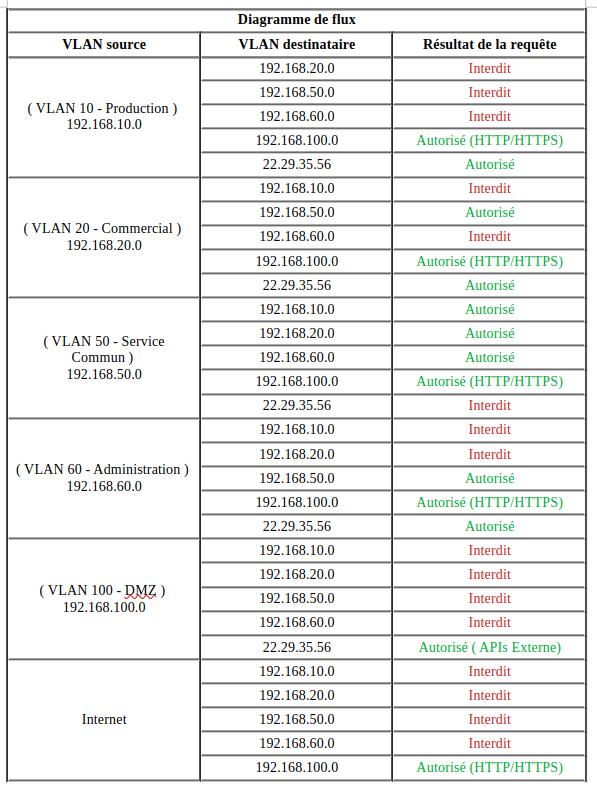
\includegraphics[width=1.0\textwidth]{Images/flux_diagram.png}
                \caption{Diagramme de Flux}
            \end{figure}
        \chapter{Schéma réseau logique}
            \begin{figure}[H]
                \centering
                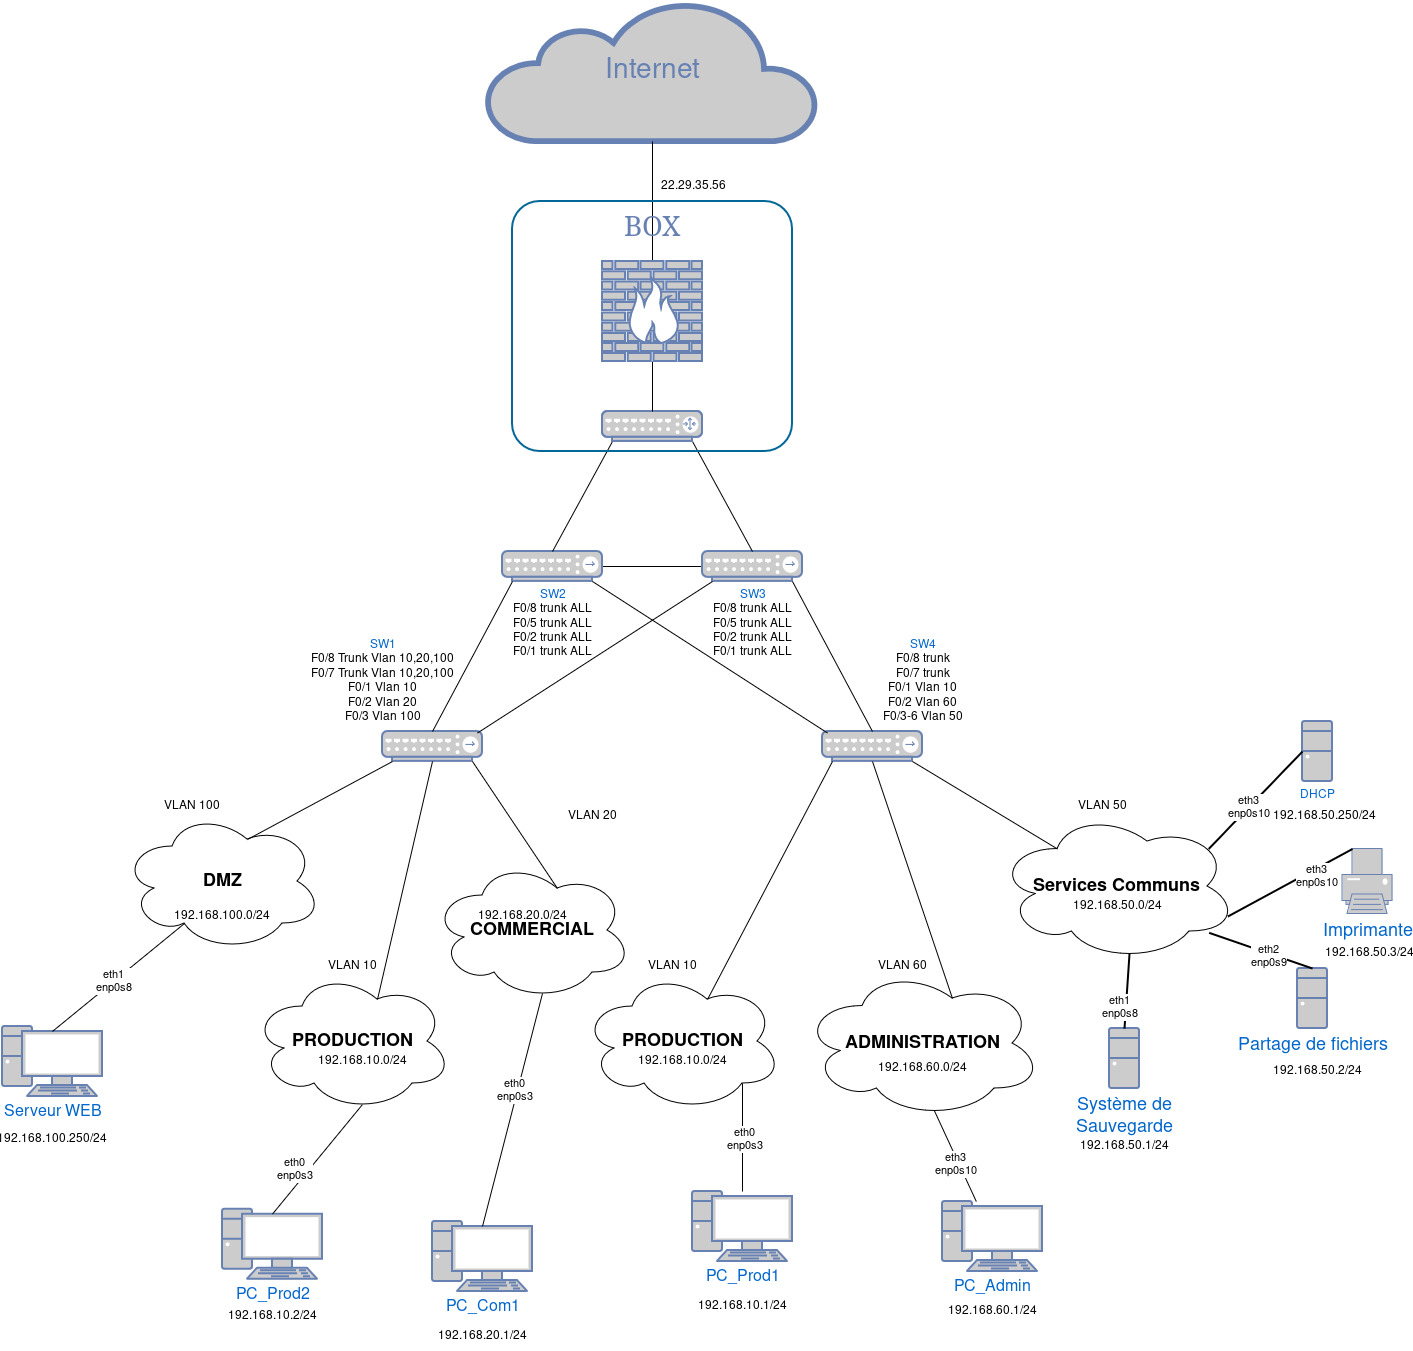
\includegraphics[width=1.0\textwidth]{Images/Schema_logique.jpg}
                \caption{Schéma réseau logique}
            \end{figure}
        \chapter{Schéma réseau physique}
            \begin{figure}[H]
                \centering
                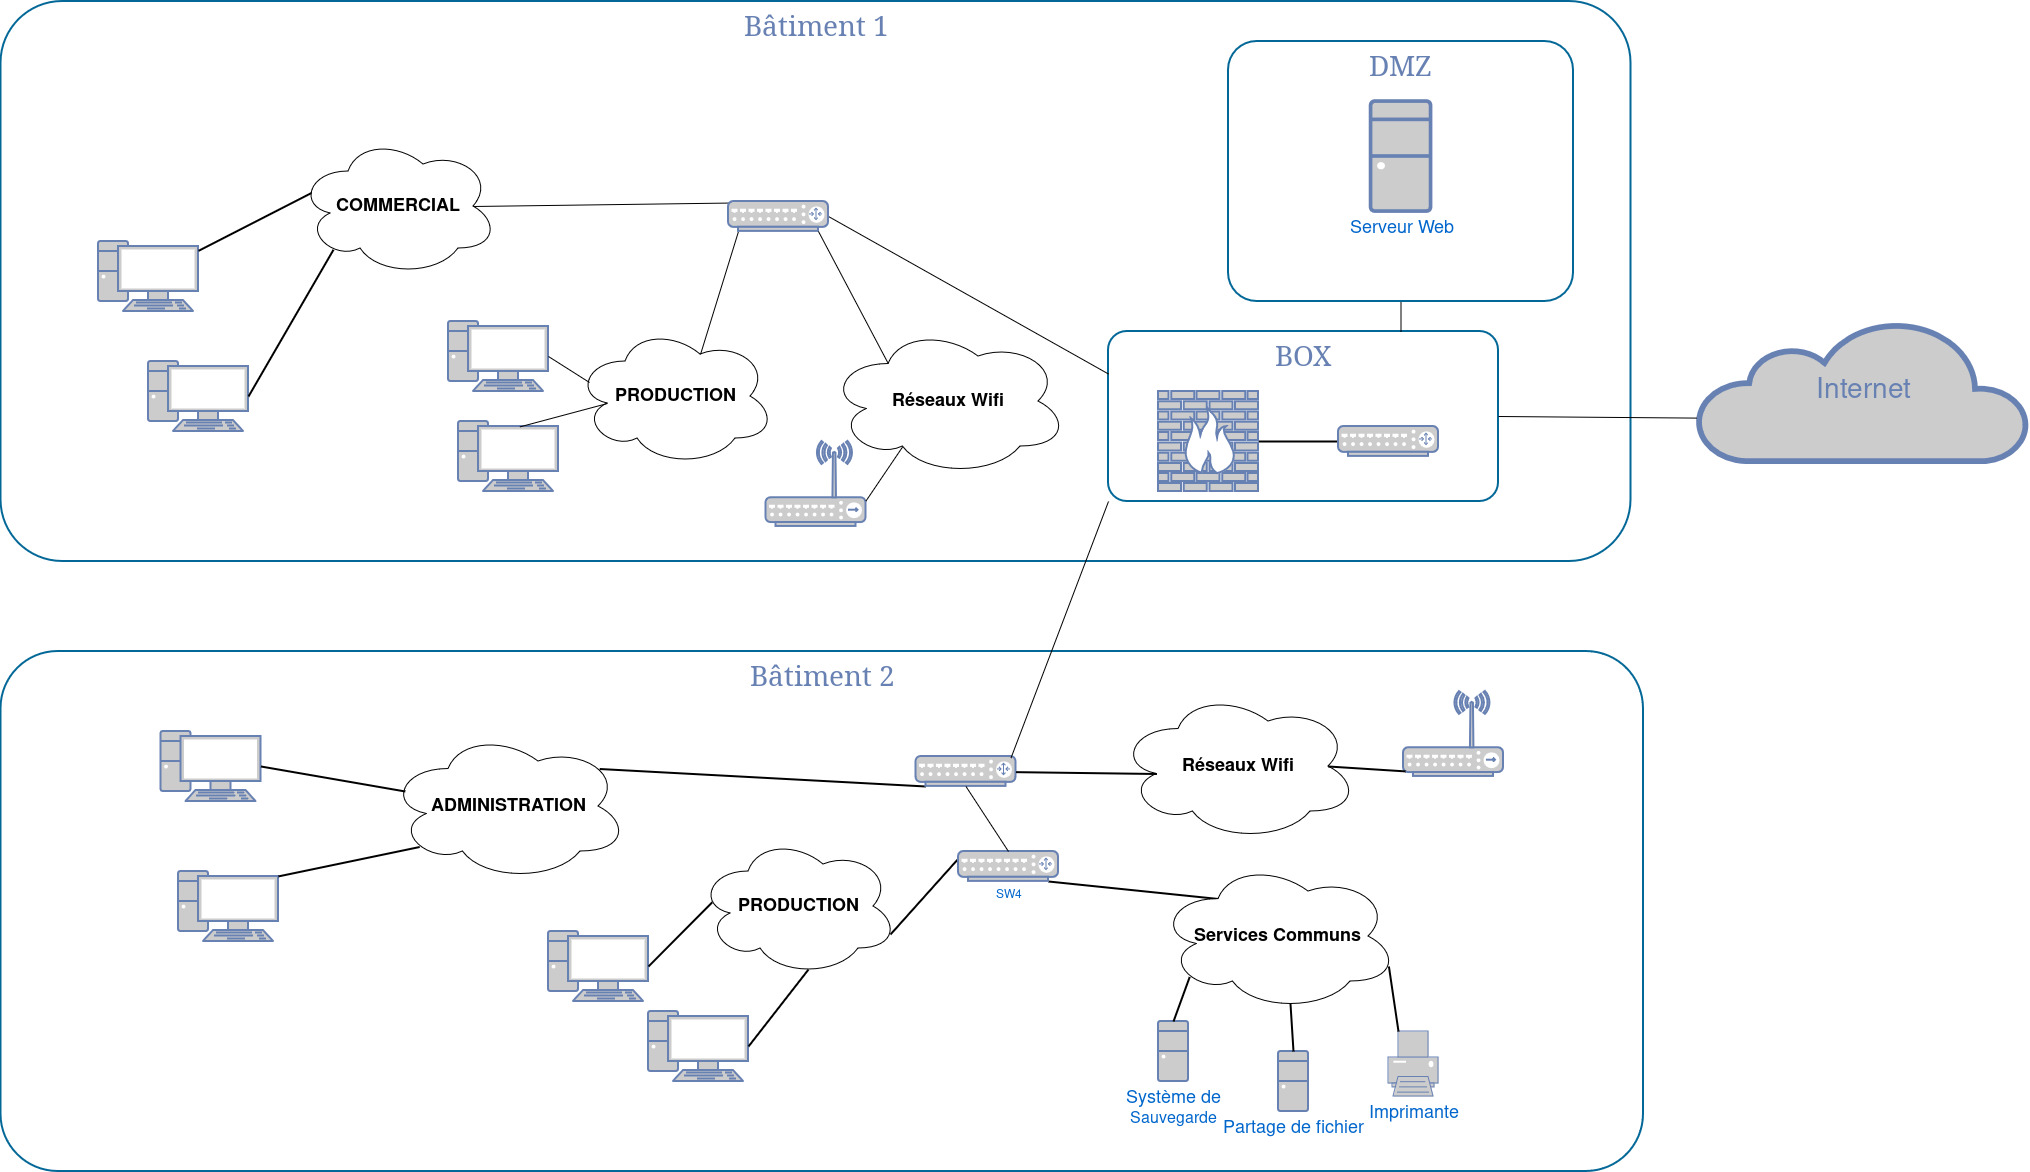
\includegraphics[width=1.2\textwidth]{Images/Schema_physique.jpg}
                \caption{Schéma réseau physique}
            \end{figure}
        \chapter{Plan d'adressage}
            \begin{figure}[H]
                \centering
                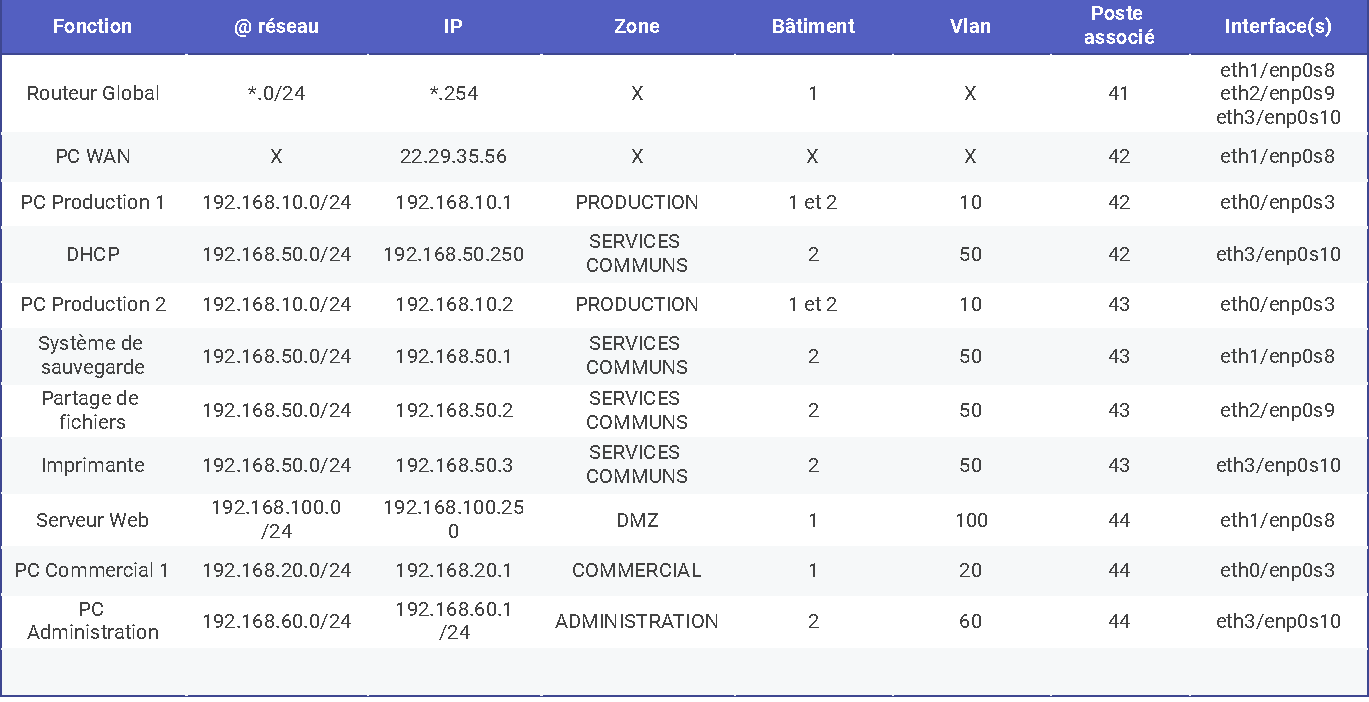
\includegraphics[width=1.2\textwidth]{Images/Plan_adressage.pdf}
                \caption{Plan d'adressage}
            \end{figure}
        \chapter{Configuration IP du routeur}
            \begin{verbatim}
1: lo: <LOOPBACK,UP,LOWER_UP> mtu 65536 qdisc noqueue state UNKNOWN 
group default qlen 1000
link/loopback 00:00:00:00:00:00 brd 00:00:00:00:00:00
inet 127.0.0.1/8 scope host lo
valid_lft forever preferred_lft forever
inet6 ::1/128 scope host 
valid_lft forever preferred_lft forever

2: enp0s3: <BROADCAST,MULTICAST> mtu 1500 qdisc noop state DOWN 
group default qlen 1000
link/ether 08:00:a0:14:11:01 brd ff:ff:ff:ff:ff:ff

3: enp0s8: <BROADCAST,MULTICAST,UP,LOWER_UP> mtu 1500 qdisc fq_codel 
state UP group default qlen 1000
link/ether 08:00:a0:14:11:02 brd ff:ff:ff:ff:ff:ff
inet 22.29.35.56/16 scope global enp0s8
valid_lft forever preferred_lft forever
inet6 fe80::a00:a0ff:fe14:1102/64 scope link 
valid_lft forever preferred_lft forever

4: enp0s9: <BROADCAST,MULTICAST,UP,LOWER_UP> mtu 1500 qdisc fq_codel 
state UP group default qlen 1000
link/ether 08:00:a0:14:11:03 brd ff:ff:ff:ff:ff:ff
inet6 fe80::a00:a0ff:fe14:1103/64 scope link dadfailed tentative 
valid_lft forever preferred_lft forever

5: enp0s10: <BROADCAST,MULTICAST,UP,LOWER_UP> mtu 1500 qdisc fq_codel 
state UP group default qlen 1000
link/ether 08:00:a0:14:11:04 brd ff:ff:ff:ff:ff:ff
inet6 fe80::a00:a0ff:fe14:1104/64 scope link dadfailed tentative 
valid_lft forever preferred_lft forever

6: enp0s9.50@enp0s9: <BROADCAST,MULTICAST,UP,LOWER_UP> mtu 1500 qdisc 
noqueue state UP group default qlen 1000
link/ether 08:00:a0:14:11:03 brd ff:ff:ff:ff:ff:ff
inet 192.168.50.254/24 scope global enp0s9.50
valid_lft forever preferred_lft forever
inet6 fe80::a00:a0ff:fe14:1103/64 scope link dadfailed tentative 
valid_lft forever preferred_lft forever

7: enp0s9.60@enp0s9: <BROADCAST,MULTICAST,UP,LOWER_UP> mtu 1500 qdisc 
noqueue state UP group default qlen 1000
link/ether 08:00:a0:14:11:03 brd ff:ff:ff:ff:ff:ff
inet 192.168.60.254/24 scope global enp0s9.60
valid_lft forever preferred_lft forever
inet6 fe80::a00:a0ff:fe14:1103/64 scope link dadfailed tentative 
valid_lft forever preferred_lft forever

8: enp0s9.10@enp0s9: <BROADCAST,MULTICAST,UP,LOWER_UP> mtu 1500 qdisc 
noqueue state UP group default qlen 1000
link/ether 08:00:a0:14:11:03 brd ff:ff:ff:ff:ff:ff
inet 192.168.10.254/24 scope global enp0s9.10
valid_lft forever preferred_lft forever
inet6 fe80::a00:a0ff:fe14:1103/64 scope link 
valid_lft forever preferred_lft forever

9: enp0s10.10@enp0s10: <BROADCAST,MULTICAST,UP,LOWER_UP> mtu 1500 qdisc 
noqueue state UP group default qlen 1000
link/ether 08:00:a0:14:11:04 brd ff:ff:ff:ff:ff:ff
inet 192.168.10.254/24 scope global enp0s10.10
valid_lft forever preferred_lft forever
inet6 fe80::a00:a0ff:fe14:1104/64 scope link dadfailed tentative 
valid_lft forever preferred_lft forever

10: enp0s10.20@enp0s10: <BROADCAST,MULTICAST,UP,LOWER_UP> mtu 1500 qdisc 
noqueue state UP group default qlen 1000
link/ether 08:00:a0:14:11:04 brd ff:ff:ff:ff:ff:ff
inet 192.168.20.254/24 scope global enp0s10.20
valid_lft forever preferred_lft forever
inet6 fe80::a00:a0ff:fe14:1104/64 scope link 
valid_lft forever preferred_lft forever

11: enp0s10.100@enp0s10: <BROADCAST,MULTICAST,UP,LOWER_UP> mtu 1500 qdisc 
noqueue state UP group default qlen 1000
link/ether 08:00:a0:14:11:04 brd ff:ff:ff:ff:ff:ff
inet 192.168.100.254/24 scope global enp0s10.100
valid_lft forever preferred_lft forever
inet6 fe80::a00:a0ff:fe14:1104/64 scope link dadfailed tentative 
valid_lft forever preferred_lft forever
            \end{verbatim}

        \chapter{Configuration du relai DHCP sur le routeur}
            \begin{verbatim}
GNU nano 6.2           /etc/default/isc-dhcp-relay                                      
# Defaults for isc-dhcp-relay initscript
# sourced by /etc/init.d/isc-dhcp-relay
# installed at /etc/default/isc-dhcp-relay by the maintainer scripts
#
# This is a POSIX shell fragment
#
# What servers should the DHCP relay forward requests to?
SERVERS="192.168.50.250"
# On what interfaces should the DHCP relay (dhrelay) serve DHCP requests?
INTERFACES="enp0s9.10 enp0s9.50 enp0s9.60 enp0s10.10 enp0s10.20 enp0s10.100"
# Additional options that are passed to the DHCP relay daemon?
OPTIONS=""
            \end{verbatim}

        \chapter{Configuration des règles d'accès du Firewall}
            \begin{verbatim}
# Politique par défaut restrictive
iptables -P INPUT DROP
iptables -P FORWARD DROP
iptables -P OUTPUT ACCEPT

# 1. Autoriser le trafic loopback
iptables -A INPUT -i lo -j ACCEPT

# 2. Autoriser les connexions établies et associées pour INPUT et FORWARD
iptables -A INPUT -m conntrack --ctstate ESTABLISHED,RELATED -j ACCEPT
iptables -A FORWARD -m conntrack --ctstate ESTABLISHED,RELATED -j ACCEPT

# 3. Bloquer la communication entre les VLANs 10, 20 et 60
iptables -A FORWARD -s 192.168.10.0/24 -d 192.168.20.0/24 -j DROP
iptables -A FORWARD -s 192.168.10.0/24 -d 192.168.60.0/24 -j DROP
iptables -A FORWARD -s 192.168.20.0/24 -d 192.168.10.0/24 -j DROP
iptables -A FORWARD -s 192.168.20.0/24 -d 192.168.60.0/24 -j DROP
iptables -A FORWARD -s 192.168.60.0/24 -d 192.168.10.0/24 -j DROP
iptables -A FORWARD -s 192.168.60.0/24 -d 192.168.20.0/24 -j DROP

# 4. Autoriser la communication de chaque VLAN (10, 20, 60) vers
le VLAN Serveur Commun (VLAN 50)
iptables -A FORWARD -s 192.168.10.0/24 -d 192.168.50.0/24 -j ACCEPT
iptables -A FORWARD -s 192.168.20.0/24 -d 192.168.50.0/24 -j ACCEPT
iptables -A FORWARD -s 192.168.60.0/24 -d 192.168.50.0/24 -j ACCEPT

# Autoriser le retour de trafic depuis le VLAN Serveur Commun vers
les VLANs internes
iptables -A FORWARD -s 192.168.50.0/24 -d 192.168.10.0/24 -j ACCEPT
iptables -A FORWARD -s 192.168.50.0/24 -d 192.168.20.0/24 -j ACCEPT
iptables -A FORWARD -s 192.168.50.0/24 -d 192.168.60.0/24 -j ACCEPT

# Autoriser seulement HTTP et HTTPS depuis les VLANs vers le serveur web
dans la DMZ (192.168.100.250)
iptables -A FORWARD -p tcp -s 192.168.10.0/24 -d 192.168.100.250 --dport 80 -j ACCEPT
iptables -A FORWARD -p tcp -s 192.168.10.0/24 -d 192.168.100.250 --dport 443 -j ACCEPT
iptables -A FORWARD -p tcp -s 192.168.20.0/24 -d 192.168.100.250 --dport 80 -j ACCEPT
iptables -A FORWARD -p tcp -s 192.168.20.0/24 -d 192.168.100.250 --dport 443 -j ACCEPT
iptables -A FORWARD -p tcp -s 192.168.60.0/24 -d 192.168.100.250 --dport 80 -j ACCEPT
iptables -A FORWARD -p tcp -s 192.168.60.0/24 -d 192.168.100.250 --dport 443 -j ACCEPT
iptables -A FORWARD -p tcp -s 192.168.50.0/24 -d 192.168.100.250 --dport 80 -j ACCEPT
iptables -A FORWARD -p tcp -s 192.168.50.0/24 -d 192.168.100.250 --dport 443 -j ACCEPT

# 6. Configurer le NAT pour rendre le serveur web accessible 
depuis l’extérieur
# Redirection du trafic HTTP
iptables -t nat -A PREROUTING -p tcp -d 22.29.35.56 --dport 80 -j DNAT --to-destination 192.168.100.250:80
# Redirection du trafic HTTPS
iptables -t nat -A PREROUTING -p tcp -d 22.29.35.56 --dport 443 -j DNAT --to-destination 192.168.100.250:443

# 7. Autoriser le trafic HTTP et HTTPS depuis tous les VLANs et depuis 
l'extérieur vers le serveur web dans la DMZ
iptables -A FORWARD -p tcp -d 192.168.100.250 --dport 80 -j ACCEPT
iptables -A FORWARD -p tcp -d 192.168.100.250 --dport 443 -j ACCEPT

# 8. Autoriser l'accès Internet pour les VLANs en activant le NAT (MASQUERADE)
iptables -t nat -A POSTROUTING -s 192.168.10.0/24 -o enp0s8 -j MASQUERADE 
iptables -t nat -A POSTROUTING -s 192.168.20.0/24 -o enp0s8 -j MASQUERADE 
iptables -t nat -A POSTROUTING -s 192.168.50.0/24 -o enp0s8 -j MASQUERADE 
iptables -t nat -A POSTROUTING -s 192.168.60.0/24 -o enp0s8 -j MASQUERADE 
iptables -t nat -A POSTROUTING -s 192.168.100.0/24 -o enp0s8 -j MASQUERADE 

# 9. Autoriser les VLANs à sortir vers Internet via le FORWARD 
iptables -A FORWARD -s 192.168.10.0/24 -o enp0s8 -j ACCEPT 
iptables -A FORWARD -s 192.168.20.0/24 -o enp0s8 -j ACCEPT 
iptables -A FORWARD -s 192.168.50.0/24 -o enp0s8 -j ACCEPT 
iptables -A FORWARD -s 192.168.60.0/24 -o enp0s8 -j ACCEPT 
iptables -A FORWARD -s 192.168.100.0/24 -o enp0s8 -j ACCEPT
            \end{verbatim}
        \chapter{Aperçu des tables IP du routeur}
            \begin{verbatim}
Chain INPUT (policy DROP)
target     prot opt source               destination         
ACCEPT     all  --  anywhere             anywhere            
ACCEPT     all  --  anywhere             anywhere             
ctstate RELATED,ESTABLISHED
Chain FORWARD (policy DROP)
target     prot opt source               destination         
ACCEPT     all  --  anywhere             anywhere             
ctstate RELATED,ESTABLISHED
DROP       all  --  192.168.10.0/24      192.168.20.0/24     
DROP       all  --  192.168.10.0/24      192.168.60.0/24     
DROP       all  --  192.168.20.0/24      192.168.10.0/24     
DROP       all  --  192.168.20.0/24      192.168.60.0/24     
DROP       all  --  192.168.60.0/24      192.168.10.0/24     
DROP       all  --  192.168.60.0/24      192.168.20.0/24     
ACCEPT     all  --  192.168.10.0/24      192.168.50.0/24     
ACCEPT     all  --  192.168.20.0/24      192.168.50.0/24     
ACCEPT     all  --  192.168.60.0/24      192.168.50.0/24     
ACCEPT     all  --  192.168.50.0/24      192.168.10.0/24     
ACCEPT     all  --  192.168.50.0/24      192.168.20.0/24     
ACCEPT     all  --  192.168.50.0/24      192.168.60.0/24     
ACCEPT     tcp  --  192.168.10.0/24      192.168.100.250      tcp dpt:http
ACCEPT     tcp  --  192.168.10.0/24      192.168.100.250      tcp dpt:https
ACCEPT     tcp  --  192.168.20.0/24      192.168.100.250      tcp dpt:http
ACCEPT     tcp  --  192.168.20.0/24      192.168.100.250      tcp dpt:https
ACCEPT     tcp  --  192.168.60.0/24      192.168.100.250      tcp dpt:http
ACCEPT     tcp  --  192.168.60.0/24      192.168.100.250      tcp dpt:https
ACCEPT     tcp  --  192.168.50.0/24      192.168.100.250      tcp dpt:http
ACCEPT     tcp  --  192.168.50.0/24      192.168.100.250      tcp dpt:https
ACCEPT     tcp  --  anywhere             192.168.100.250      tcp dpt:http
ACCEPT     tcp  --  anywhere             192.168.100.250      tcp dpt:https
ACCEPT     all  --  192.168.10.0/24      anywhere            
ACCEPT     all  --  192.168.20.0/24      anywhere            
ACCEPT     all  --  192.168.50.0/24      anywhere            
ACCEPT     all  --  192.168.60.0/24      anywhere            
ACCEPT     all  --  192.168.100.0/24     anywhere            
Chain OUTPUT (policy ACCEPT)
target     prot opt source               destination         
            \end{verbatim}
    \end{appendices}
        
\end{document} 